\newcommand{\of}{\texttt{.o}~}

\lab{Interfacing With Other Programming Languages Using Cython}{Interfacing With Other Programming Languages Using Cython}
\label{lab:cythonwrap}

\objective{Learn to interface with object files using Cython. This lab should be worked through on a machine that has already been configured to build Cython extensions using gcc or MinGW.}

Suppose you are writing a program in Python, but would like to call code written in another language.
Perhaps this code has already been debugged and heavily optimized, so you do not want to simply re-implement the algorithm in Python or Cython.
In technical terms, you want Python to \emph{interface} (or communicate) with the other language.
For example, NumPy's linear algebra functions call functions from LAPACK and BLAS, which are written in Fortran.

One way to have Python interface with C is to write a Cython \emph{wrapper} for the C function.
The wrapper is a Cython function that calls the C function. 
This is relatively easy to do because Cython compiles to C.
From Python, you can call the wrapper, which calls the C function (see Figure TODO).
In this lab you will learn how to use Cython to wrap a C function.

\section*{Wrapping with Cython: an overview}
When you use Cython to wrap a C function, you just write a Cython function that calls the C function.
To actually do this, we need to understand a little bit more about how C works.

After you write a program in C, you pass it to a compiler.
The compiler turns your C code into machine code, i.e., instructions that your computer can read.
The output of the compiler is an \emph{object file}.

In our scenario, we have C code defining a single function that we would like to wrap in Cython.
This C code has already been compiled to an object file.
The protocol for calling the C code from Cython is similar to calling it from C:
\begin{enumerate}
\item we need to \emph{include a header file} for the C code in our Cython code, and
\item we must \emph{link to the object file} compiled from the C code when we compile the Cython code.
\end{enumerate}

A \emph{header} for a file contains the declaration of the function defined in the file.
We include the header in the Cython code so that the compiler can check that the function is called with the right number and types of arguments.
Then, when we tell the compiler to \emph{link to} the object file, we simply tell it where to find the instructions defining the function declared in the header.

The Cython code will compile to a second object file.
This object file defines a module that can be imported into Python. See Figure \ref{fig:cython_flowchart}.

%TODO: make figure
\begin{figure}
\begin{tikzpicture}[dot/.style={circle,fill=black,minimum size=3pt,inner sep=0pt,
            outer sep=-1pt}, >=stealth', thick]

\node[draw, minimum height=1.5cm, minimum width=3cm, align=center](ctri1)
	[]{\Large{ctridiag.h} \\ {\small declare \texttt{ctridiag()}}};

\node[draw, minimum height=1.5cm, minimum width=3cm, align=center, node
	distance=2.5cm](ctri2)[below of=ctri1]{\Large{ctridiag.c} \\ {\small define \texttt
	{ctridiag()}}};

\node[draw, minimum height=1cm, minimum width=2cm, align=center, node
	distance=2.2cm, color=white!40!black](ctri3)[below of=ctri2]{COMPILE};

\node[draw, minimum height=.7cm, minimum width=3cm, align=center, node
	distance=1.9cm](ctri4)[below of=ctri3]{ \Large{ctridiag.o} \\{\small object file callable} \\ {\small from C}};

%\node[draw, minimum height=1cm, minimum width=3cm, align=center, node
%	distance=.85cm](ctri5)[below of=ctri4]{object file  \\ callable by C};

\draw[-, color=white!40!black](ctri2)--(ctri3);
\draw[->, shorten >=3pt,color=white!40!black](ctri3)--(ctri4);

\node[draw, minimum height=1.5cm, minimum width=3cm, align=center, node
	distance=7cm](ctri6)[right of=ctri1]{\Large{cython\_ctridiag.pyx}
	 \\ {\small define \texttt{cytridiag()}}};

\node[draw, minimum height=1cm, minimum width=2cm, align=center, node
	distance=3.3cm,color=white!40!black](ctri7)[below of=ctri6]{COMPILE};

\node[draw, minimum height=1.5cm, minimum width=3cm, align=center, node
	distance=3.3cm](ctri8)[below of=ctri7]{\Large{ctridiag.so} \\ {\small object file 
	callable} \\ {\small from Python}};

\draw[-, color=white!40!black](ctri6)--(ctri7);
\draw[->, shorten >=3pt,color=white!40!black](ctri7)--(ctri8);
\draw[->, dashed, shorten >=3pt,color=white!40!black](1.5,-6.95)--(6, -3.3);
\draw[->, shorten >=3pt,color=white!40!black](ctri1)--(ctri6);

\node[draw, minimum height=.7cm, minimum width=1cm, align=center, node
	distance=3.1cm,color=white!40!black, fill=white](include)[right of=ctri1]
	{INCLUDE};

\node[draw, minimum height=.7cm, minimum width=1cm, align=center, node
	distance=5.8cm,color=white!40!black, fill=white](include)at(3.7,-5.15){LINK};

\end{tikzpicture}
\caption{This diagram shows the relationships between the files used to write a Cython wrapper for \li{ctridiag()}.
In fact, the Cython file \texttt{cython\_ctridiag.pyx} compiles first to C code and then to the shared object file, but we have omitted this step from the diagram.}
\label{fig:cython_flowchart}
\end{figure}

\section*{Wrapping with Cython: an example}
As an example, we will wrap the C function \texttt{ctridiag()} below.
This function computes the solution to a tridiagonal system $A\v = \x$.
Its parameters are pointers to four 1-D arrays, which satisfy the following:
\begin{itemize}
\item Arrays \li{a} and \li{c} have length \li{n-1} and contain the first subdiagonal and superdiagonal of $A$, respectively.
\item Arrays \li{b} and \li{x} have length \li{n} and represent the main diagonal of $A$ and $\x$, respectively.
\end{itemize}
The array \li{c} is used to store temporary values and \li{x} is transformed into the solution of the system.

\lstinputlisting[style=fromfile, language=C, name=ctridiag.c]{./ctridiag/ctridiag.c}

This terminal command tells the C-compiler gcc to compiles \texttt{ctridiag.c} to an object file \texttt{ctridiag.o}.

\begin{lstlisting}
>>> gcc -fPIC -c ctridiag.c -o ctridiag.o
\end{lstlisting}
The \texttt{-fPIC} option is required because we will later link to this object file when compiling a shared object file.
The \texttt{-c} flag prevents the compiler from raising an error even though \texttt{ctridiag.c} does not have a \li{main} function.




\subsection*{Write a header for \texttt{ctridiag.c}}

The header file essentially contains a function declaration for \li{ctridiag()}.
It tells Cython how to use the object file \li{ctridiag.o}.
\lstinputlisting[style=fromfile, language=C, name=ctridiag.h]{./ctridiag/ctridiag.h}

\subsection*{Write a Cython wrapper}
Next we write a Cython file containing a function that ``wraps'' \li{ctridiag()}.
This file must include the header we wrote in the previous step.

\lstinputlisting[style=fromfile, language=Python, name=cython_ctridiag.pyx]{./ctridiag/cython_ctridiag.pyx}

Some comments on this code are in order. 
First, including the header for \li{ctridiag()} allows us to call this function even though it was not defined in this file.
This is a little like importing NumPy at the start of your Python script.

Second, the arguments of the Cython function \li{cytridiag()} are not in bijection with the arguments of \li{ctridiag()}.
In fact, Cython does not need to know the size of the NumPy arrays it accepts as inputs because these arrays are objects that carry that information with them.
We extract this information and pass it to the C function inside the Cython wrapper.

However, it is possible to unintentionally access memory outside of an array by calling this function.
For example, suppose the input arrays \li{a}, \li{b}, \li{c}, and \li{x} are of sizes 4, 5, 3, and 5.
Since \li{x} is used to determine the size of the system, the function \li{ctridiag()} will expect \li{c} to have length 4.
At some point, \li{ctridiag()} will likely try to read or even write to the 4th entry of \li{c}.
This address does exist in memory, but it does not contain an entry of \li{c}!
Therefore, this function must be called by a responsible user who knows the sizes of her arrays.
Alternatively, you could check the sizes of the arrays in the Cython wrapper before passing them to the C function.

Finally, the C function expects a parameter \li{double* a}, meaning that \li{a} is a \emph{pointer to} (i.e., the address of) a \li{double}.
The funtion \li{ctridiag()} expects this double to be the first entry of the array \li{a}.
So instead of passing the object \li{a} to \li{ctridiag()}, we find the first entry of \li{a} with \li{a[0]}, and then take its address with the \li{&} operator.





\subsection*{Compile the Cython wrapper}

Now we can compile \texttt{cython\_ctridiag.pyx} to build the Python extension.
The following setup file uses distutils to compile the Cython file, and may be run on Windows, Linux, or Macintosh-based computers.
Notice that in line 28, we link to the existing object file \texttt{ctridiag.o}.

\lstinputlisting[style=fromfile, language=Python, name=ctridiag_setup_distutils.py]{./ctridiag/ctridiag_setup_distutils.py}

This setup file can be called from the command line with the following command.
\begin{lstlisting}[style=ShellInput]
python ctridiag_setup_distutils.py build_ext --inplace
\end{lstlisting}
The \texttt{--inplace} flag tells the script to compile the extension in the current directory.
The appendix at the end of this lab contains setup files that build the Python extension by hand on various operating systems.





\subsection*{Test the Python extension}
After running the setup file, you should have a Python module called \li{cython_cytridiag} that defines a function \li{cytridiag()}.
You can import this module into IPython as usual.
However, if you modify \li{ctridiag()} and then try to recompile the extension, you may get an error if the module is currently in use.
Hence, if you are frequently recompiling your extension, it is wise to test it  with a script.

The following script tests the module \li{cython_cytridiag}.

\lstinputlisting[style=fromfile, language=Python, name=ctridiag_test.py]{./ctridiag/ctridiag_test.py}

\begin{warn}
When passing arrays as pointers to C or Fortran functions, be \emph{absolutely sure} that the array being passed is contiguous.
This means that the entries of the array are stored in \emph{adjacent} entries in memory.
Passing one of these functions a strided array will result in out of bounds memory accesses and could crash your computer.
For an example of how to check an array is contiguous in a Cython wrapper, see Problem \ref{prob:c_wrap}.
\end{warn}



\section*{Another example}
%TODO: replace the C function for this problem with one that implements Monte Carlo integration


The C function \li{cssor()} below implements the Successive Over Relaxation algorithm for solving Laplace's equation, which in two dimensions is
\[
\frac{\partial^2 F}{\partial x^2} + \frac{\partial^2 F}{\partial y^2} = 0.
\]
In the Successive Over Relaxation algorithm, an input array is iteratively modified until it converges to the solution $F(x,y)$.

\lstinputlisting[style=fromfile, language=C, name=cssor.c]{./cssor/cssor.c}

The function \li{cssor()} accepts the following inputs.
\begin{itemize}
\item $U$ is a pointer to a Fortran-contiguous 2-D array of double precision numbers.
\item $m$ is an integer storing the number of rows of $U$.
\item $n$ is an integer storing the number of columns of $U$.
\item $\omega$ is a double precision floating point value between $1$ and $2$.
The closer this value is to $2$, the faster the algorithm will converge, but if it is too close the algorithm may not converge at all.
For this lab just use $1.9$.
\item tol is a floating point number storing a tolerance used to determine when the algorithm should terminate.
\item maxiters is an integer storing the maximum allowable number of iterations.
\item info is a pointer to an integer.
This function will set info to $0$ if the algorithm converged to a solution within the given tolerance.
It will set info to $1$ if it did not.
\end{itemize}



\begin{problem}\label{prob:c_wrap}
Wrap \li{cssor()} so it can be called from Python, following these steps.
\begin{enumerate}
\item Write a C header for \li{cssor.c}.
\item Write a Cython wrapper \li{cyssor()} for the function \li{cssor()} as follows.
    \begin{enumerate}
    \item Have \li{cyssor()} accept parameters \li{tol} and \li{maxiters} that default to $10e^{-8}$ and 10,000, respectively.
    What other arguments does \li{cyssor()} need to accept?
    \item Check that the input \li{U} is a C-contiguous array (this means that the array is stored in a certain way in memory).
    You can check if \li{U} is C-contiguous with the code \li{U.is_c_contig()}, which returns a Boolean value.
    If \li{U} is not C-contiguous, raise a ValueError as follows:
    \begin{lstlisting}
    raise ValueError('Input array U is not C-contiguous')
    \end{lstlisting}
    When raising a ValueError, you may replace the string \li{'Input array U is not C-contiguous'} with any desired text.
    For more about errors and exceptions in Python, see \url{https://docs.python.org/2/tutorial/errors.html}.
    \item Raise a ValueError if \li{cssor()} fails to converge---i.e., if \li{cssor()} sets \li{info} to 1.
    \end{enumerate}
\item Compile \li{cssor.c} to an object file and compile your Cython wrapper to a Python extension. 
Be aware that you may compile \li{cssor.c} correctly and still receive warnings from the compiler.
\item Write a test script for your Cython function.
    \begin{enumerate}
    \item You can run the function with the following code.
    \begin{lstlisting}
	import numpy as np
	from cython_fssor import cyssor
	resolution = 501
	U = np.zeros((resolution, resolution))
	X = np.linspace(0, 1, resolution)
	U[0] = np.sin(2 * np.pi * X)
	U[-1] = - U[0]
	cyssor(U, 1.9)
	\end{lstlisting}
    \item Have your test script run the code above and plot the modified array \li{U} on the domain $[0,1]\times[0, 1]$. 
    Note that $U$ is a $501\times 501$ array.
    Your plot should look like Figure \ref{fig:solution}.
    \end{enumerate}
\end{enumerate}

%TODO: mayavify this plot.
\begin{figure}[H]
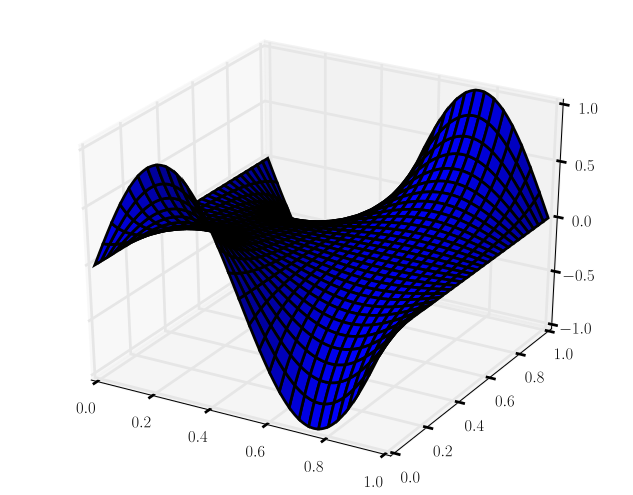
\includegraphics[width=\textwidth]{solution.png}
\caption{Correct output for the test script of Problem \ref{prob:c_wrap}.}
\label{fig:solution}
\end{figure}

\end{problem}

\section*{Wrapping a Fortran function (Optional)}
We can also use Cython to wrap Fortran.
As an example, we will wrap the Fortran function below, which implements the same algorithm as \li{ctridiag()}.

We have used the C library \li{iso_c_binding} to make the function accept pointers to native C types.
If we were wrapping a function or subroutine that we did not write ourselves, we would have to define a Fortran function that uses the \li{iso_c_binding} library to accept pointers from C and then uses the values it receives to call the original function.
\lstinputlisting[style=fromfile, language=Fortran, name=ftridiag.f90]{./ftridiag/ftridiag.f90}

\begin{warn}
When interfacing between Fortran and C, you will have to pass pointers to \emph{all} the variables you send to the Fortran function as arguments.
Passing a variable directly will probably crash Python.
\end{warn}

\subsection*{Write a header for \texttt{ftridiag.f90}}
Here is a header that tells C how to interface with the function we have just defined.
\lstinputlisting[style=fromfile, language=C, name=ftridiag.h]{./ftridiag/ftridiag.h}

To compile \li{ftridiag.f90} to an object file you can run the following command in your command line:
\begin{lstlisting}[style=ShellInput]
gfortran -fPIC -c ftridiag.f90 -o ftridiag.o
\end{lstlisting}

\subsection*{Write a Cython wrapper, compile, and test it}
The Cython wrapper for this function is analogous to \li{cython_ctridiag.pyx}, except that every variable passed to \li{ftridiag} should be a pointer.
Aside from the use of gfortran instead of gcc, the rest of the compilation and testing process is entirely the same.
The setup files specific to Windows and Linux, the setup file using distutils, and the test script are included in this lab folder.

\begin{warn}
Fortran differs from C in that the columns of arrays are stored in contiguous blocks of memory instead of the rows.
The default for NumPy and for C arrays is to have rows stored in contiguous blocks, but in NumPy this varies.
You should make sure any code passing arrays between Fortran, C, and NumPy addresses this discrepancy.
Though by default Fortran assumes arrays are arranged in Fortran-order, for many routines you can specify whether to act on an array or its transpose.
\end{warn}

\begin{info}
The function \li{ftridiag()} may seem unusual because it is a Fortran function that is callable from C.
In fact, this is not an uncommon scenario.
Many larger Fortran libraries (for example, LAPACK) provide C wrappers for all their functions.
\end{info}

\subsection*{Another example}

Here is a Fortran implementation of the Successive Over Relaxation algorithm for solving Laplace's equation.
This function is the Fortran equivalent of \li{cssor.c}.
Its parameters are the same, with the exception that all parameters are \emph{points} to the values they reference.

\lstinputlisting[style=fromfile, language=Fortran, name=fssor.f90]{./fssor/fssor.f90}

\begin{problem}
Imitate Problem \ref{prob:c_wrap} to wrap \li{fssor()} with Cython.
\end{problem}


\section*{Appendix: compiling C extensions for Python}
If you know more about compilers, you may find it enlightening to manually compile a C extension for Python.
Here we show how to manually compile \texttt{cython\_ctridiag.pyx} on Windows, Linux, and Macintosh machines.

On Windows, using the compiler MinGW (a version of gcc for windows), the compilation can be performed by running the following setup file.

\lstinputlisting[style=fromfile, language=Python, name=ctridiag_setup_windows64.py]{./ctridiag/ctridiag_setup_windows64.py}

The following file works on Linux and Macintosh machines using gcc.

\lstinputlisting[style=fromfile, language=Python, name=ctridiag_setup_linux.py]{./ctridiag/ctridiag_setup_linux.py}
\end{document}
